\section{Methodology}
\sloppy

\subsection{Proposed Solution}
To address the navigation challenges in GPS-restricted environments, the proposed solution implements a tightly-coupled, real-time Visual-Inertial Navigation System (VINS) utilizing the ORB-SLAM3 framework in RGBD-Inertial mode. This architecture leverages an NVIDIA Jetson Orin NX companion computer for high-performance processing and an Orbbec Gemini 2L camera to provide synchronized RGB, depth, and 200Hz IMU data. By utilizing aligned depth maps, the system establishes an absolute metric scale from the initial frame, effectively eliminating the scale ambiguity and initialization delays common in monocular systems. The software pipeline, orchestrated via ROS 2 Humble, integrates a custom VIO Bridge to manage frame transformations and coordinate alignment, ensuring the SLAM-derived poses are accurately fused into the Pixhawk 6X Pro flight controller's EKF2 estimator through the MAVROS bridge for stable, closed-loop autonomous flight

\subsection{System Architecture}
The VIO system follows a modular pipeline architecture consisting of four ROS 2 nodes spread across three custom packages, orchestrated to provide seamless state estimation. The pipeline processes sensor data through a well-defined chain: raw camera and IMU data $\rightarrow$ visual SLAM $\rightarrow$ frame transformation and heading correction $\rightarrow$ flight controller integration \cite{ros2_humble,mavros_wiki,px4_user_guide}.

\begin{figure}[H]
    \centering
    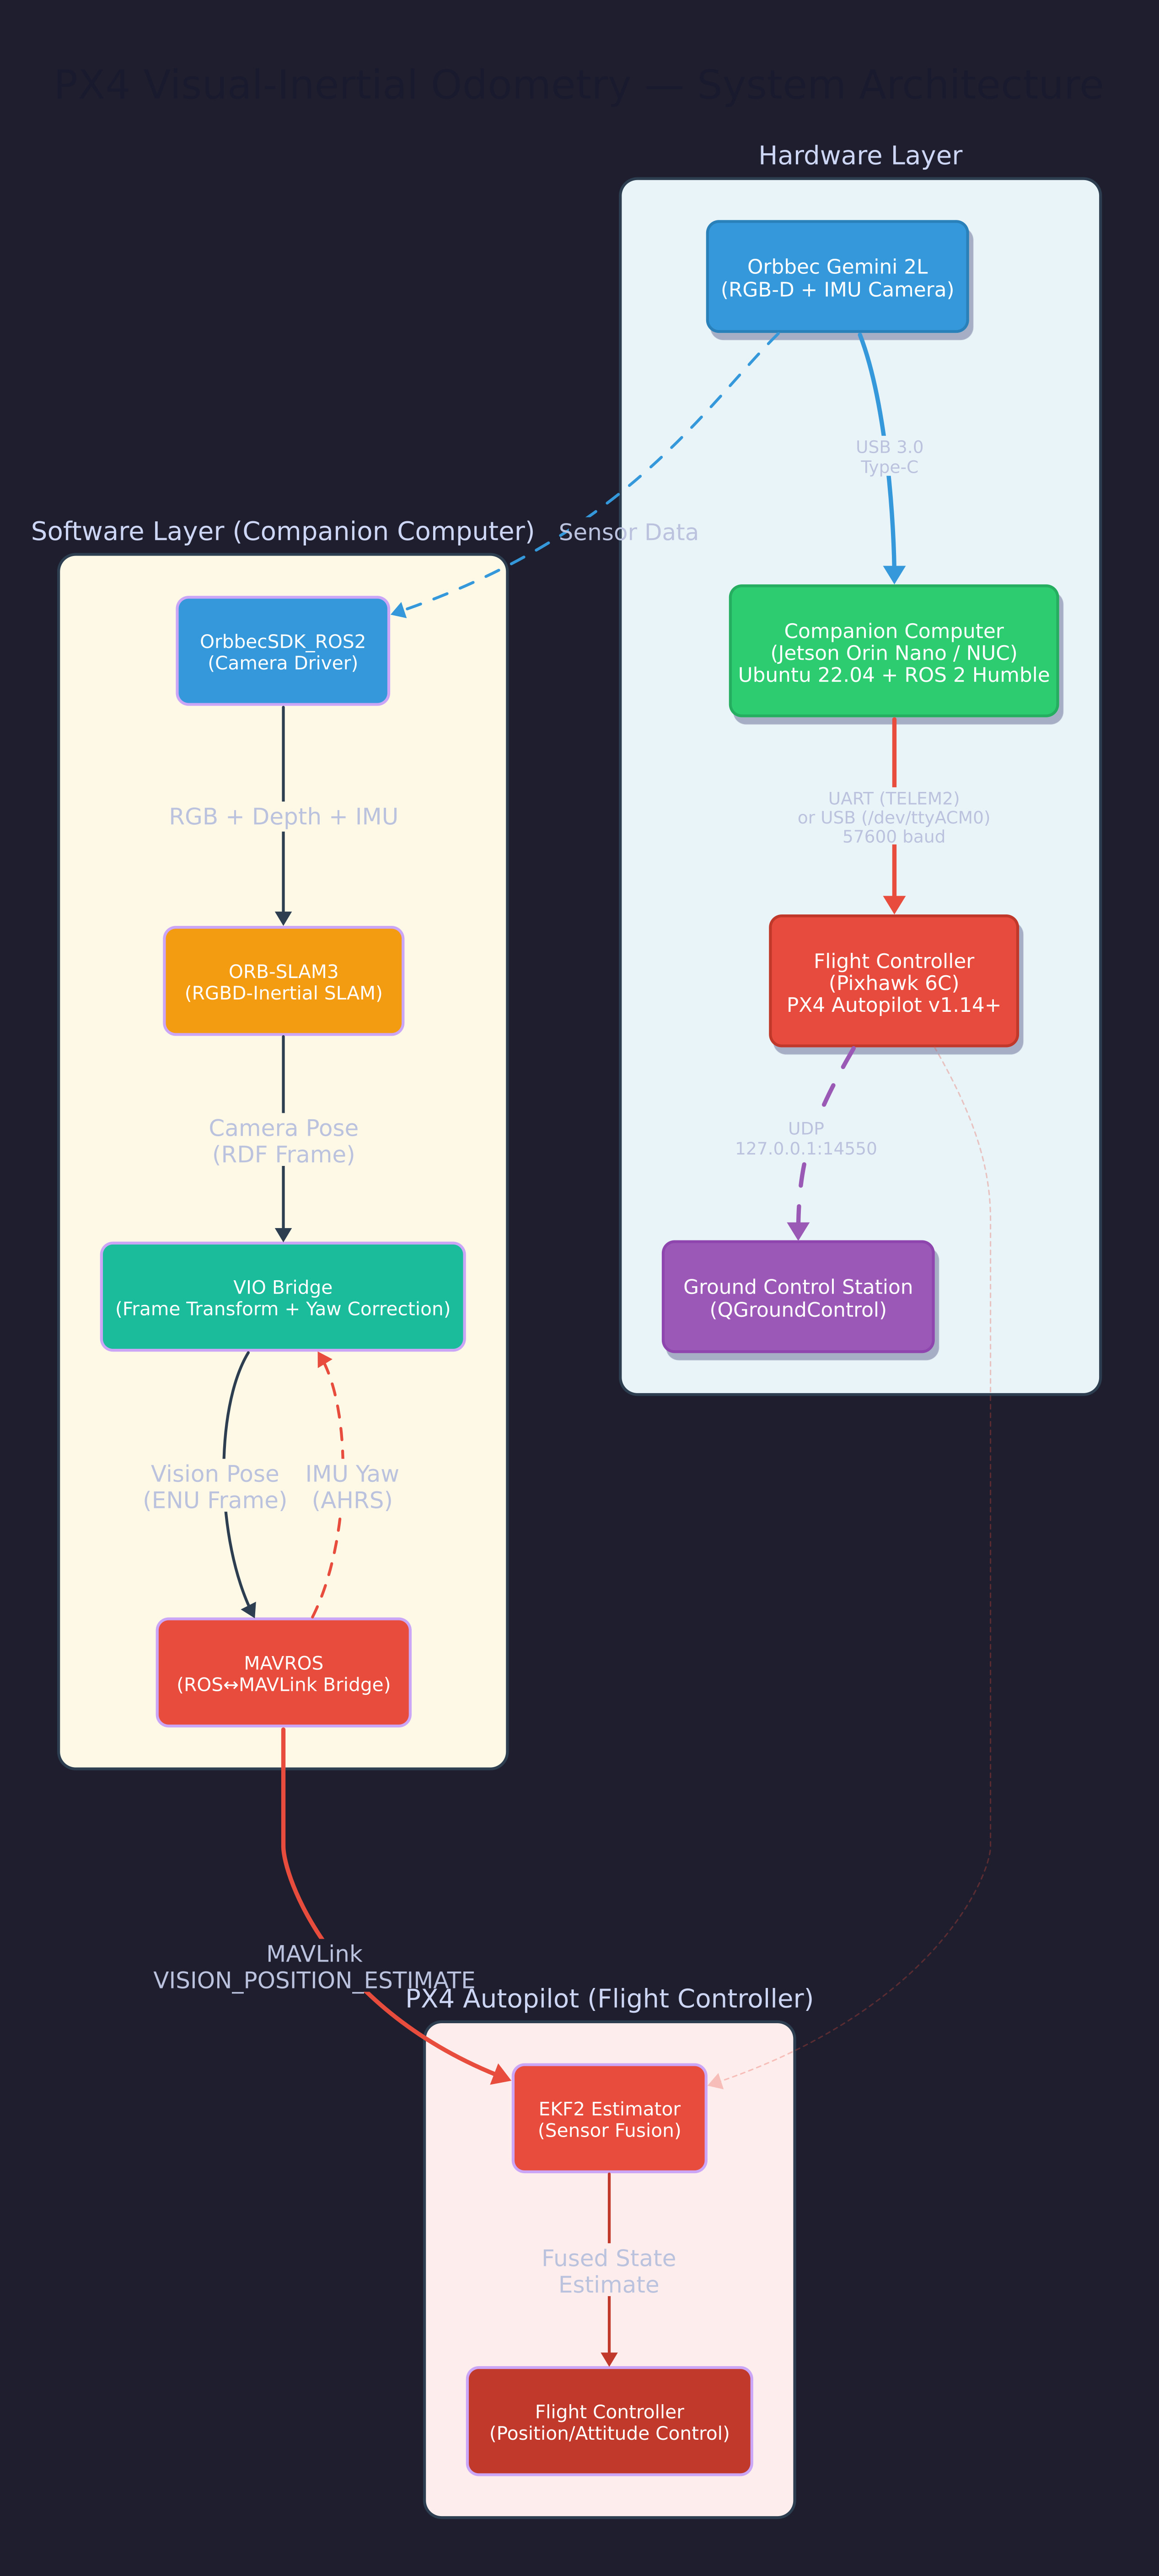
\includegraphics[width=\linewidth,height=0.75\textheight,keepaspectratio]{images/01_system_architecture.jpg}
    \caption{System architecture overview of the ROS~2-based VIO/navigation stack.}
    \label{fig:system_architecture}
\end{figure}

The architecture is deliberately focused on the core VIO pipeline, prioritizing robustness and low latency over feature complexity. Each node has a single, well-defined responsibility, making the system easier to debug, maintain, and validate in real flight conditions.


\begin{table}[H]
\centering
\scriptsize % reduces font size
\caption{ROS Nodes}
\resizebox{\textwidth}{!}{%
\begin{tabular}{|p{2.8cm}|p{2.6cm}|p{6.6cm}|p{4.2cm}|}
\hline \textbf{Node} & \textbf{Package} & \textbf{Role} & \textbf{Key Output} \\

\hline Orbbec Camera Node & OrbbecSDK\_ROS2 & Publishes synchronized RGB, Depth, and IMU data from the Gemini 2L camera \cite{orbbec_ros2_sdk} & RGB images (30Hz), Depth maps (30Hz), IMU (200Hz) \\

\hline ORB-SLAM3 Node & orbslam3\_ros2 & Performs RGBD-Inertial SLAM --- extracts features, fuses IMU, and estimates camera pose & 6-DOF Camera Pose in gravity-aligned world \\

\hline VIO Bridge Node & vio\_bridge & Transforms SLAM pose (RDF$\rightarrow$ENU), applies yaw correction, monitors drift, detects resets & Corrected Body Pose in ENU frame \\

\hline MAVROS Node & mavros & Bridges ROS 2 to PX4 via MAVLink --- converts ENU$\rightarrow$NED and sends vision pose estimates & VISION\_POSITION\_ESTIMATE MAVLink message \\

\hline \end{tabular}}
\label{tab:ros_nodes}
\end{table}

\subsection{Hardware Platform}
The system is built on the Holybro Jetson Pack — an integrated carrier board solution that combines the NVIDIA Jetson Orin NX 16GB module with the Holybro Pixhawk 6X Pro flight controller \cite{holybro_jetson_pack,jetson_orin_nx_datasheet,pixhawk6x_datasheet}. This provides a compact, flight-ready package with direct inter-processor communication, eliminating the need for external wiring between the companion computer and the autopilot \cite{holybro_jetson_pack}.

\begin{table}[H]
\centering
\scriptsize
\caption{Hardware Components}
\setlength{\tabcolsep}{3pt}% tighten columns (helps keep height down)
\renewcommand{\arraystretch}{0.9}% tighten row spacing (helps keep height down)
\resizebox{\textwidth}{!}{%
\begin{tabular}{|p{3.0cm}|p{3.2cm}|p{7.3cm}|p{7.3cm}|}
\hline
\textbf{Component} & \textbf{Model} & \textbf{Specification} & \textbf{Reason for Choosing} \\

\hline
Companion Computer & NVIDIA Jetson Orin NX 16GB (Holybro Jetson Pack) &
Ubuntu 22.04, ROS 2 Humble, 16GB LPDDR5 RAM, 8-core ARM Cortex-A78AE, 1024-core Ampere GPU, 100 TOPS AI\cite{jetson_orin_nx_datasheet} &
Provides high-performance onboard GPU acceleration required for real-time SLAM, visual processing, and autonomous navigation \\

\hline
RGB-D Camera & Orbbec Gemini 2L &
1280$\times$800 RGB @ 30fps, aligned depth @ 30fps, on-board IMU @ 200Hz, 100\,mm stereo baseline\cite{orbbec_gemini2l_datasheet} &
Provides synchronized RGB, depth, and inertial data required for accurate visual-inertial SLAM \\

\hline
Flight Controller & Holybro Pixhawk 6X Pro (PX4 v1.14+) &
STM32H7 processor, triple redundant IMU, EKF2 estimator, MAVLink telemetry\cite{pixhawk6x_datasheet} &
Provides reliable flight control and supports external vision-based position estimation for GPS-denied navigation \\

\hline
Battery & CNHL LiPo 4S 5200mAh &
14.8\,V nominal voltage, 5200mAh capacity, high discharge rate LiPo battery\cite{cnhl_5200mah_datasheet} &
Provides sufficient power capacity and stable voltage supply for flight controller, companion computer, and onboard sensors \\

\hline
Drone Frame & S500 Quadcopter Frame &
500\,mm wheelbase, lightweight composite frame, supports quad-motor configuration\cite{s500_frame_specs} &
Provides stable structure with sufficient payload capacity and mounting space for onboard computing and sensing hardware \\

\hline
Motors (×4) & 2212 920KV Brushless Motors &
920KV rating, supports 2--4S LiPo, max current $\sim$18A, thrust $\sim$500g per motor\cite{motor_2212_920kv} &
Provides sufficient thrust-to-weight ratio and efficient performance for stable autonomous flight \\

\hline
Propellers (×4) & 9450 Propellers &
9.4-inch diameter, 5.0-inch pitch, compatible with 2212 motors\cite{propeller_9450} &
Provides efficient thrust generation and aerodynamic stability for quadcopter operation \\

\hline
Electronic Speed Controller (×4) & SimonK 30A ESC &
30A continuous current, supports 2--4S LiPo, fast response firmware\cite{motor_2212_920kv} &
Provides reliable and precise motor speed control required for stable flight and attitude control \\

\hline
RF Receiver & RadioMaster ER6 Receiver &
2.4\,GHz ExpressLRS receiver, 6 channels, low latency, long range\cite{radiomaster} &
Provides reliable manual control capability for testing, safety override, and system calibration \\

\hline
WiFi Telemetry Module & CUAV PW-Link Module &
2.4\,GHz WiFi telemetry, MAVLink support, UART interface, low latency communication\cite{cuav_pwlink_datasheet} &
Enables wireless telemetry communication between UAV and ground station for monitoring and control \\
\hline

\end{tabular}}
\label{tab:hardware_components}
\end{table}


The Holybro Jetson Pack carrier board provides a direct UART connection between the Jetson Orin NX and the Pixhawk 6X Pro, removing the need for USB adapters or external serial converters. The 16GB of LPDDR5 RAM ensures headroom for ORB-SLAM3's memory-intensive map management alongside camera processing and ROS 2 overhead.

\subsection{Software Stack}
The software environment and key dependencies are as follows:

\begin{table}[H]
\centering
\scriptsize
\caption{Software Stack}
\resizebox{\textwidth}{!}{%
\begin{tabular}{|p{3.2cm}|p{4.2cm}|p{9.8cm}|}
\hline \textbf{Software} & \textbf{Version} & \textbf{Purpose} \\

\hline Ubuntu & 22.04 LTS (Jammy) & Base operating system (JetPack 6.x compatible) \cite{ubuntu_2204} \\

\hline ROS 2 & Humble Hawksbill & Middleware framework for inter-node communication \cite{ros2_humble} \\

\hline OrbbecSDK\_ROS2 & Latest & Camera driver with synchronized IMU output \cite{orbbec_ros2_sdk} \\

\hline MAVROS & ROS 2 Humble release & MAVLink bridge to PX4 flight controller \cite{mavros_wiki} \\

\hline PX4 Autopilot & v1.14+ & Flight controller firmware with EKF2 vision fusion \cite{px4_user_guide} \\

\hline CUDA Toolkit & 11.x / 12.x & Enables GPU acceleration for SLAM, deep learning, and image processing \\

\hline OpenCV & 4.x (with CUDA) & Image processing and feature extraction with GPU acceleration \\

\hline QGroundControl & v4.x & Ground control station for UAV configuration, telemetry, and mission testing \\

\hline
\end{tabular}}
\label{tab:software_stack}
\end{table}

\subsection{Sensor Data Aquisition}
The Orbbec Gemini 2L camera provides all perceptual data for the SLAM system through three synchronized data streams \cite{orbbec_gemini2l_datasheet}. The camera's on-board IMU eliminates the need for an external inertial sensor, simplifying the hardware setup and reducing extrinsic calibration complexity \cite{orbbec_gemini2l_datasheet}.

\begin{figure}[H]
    \centering
    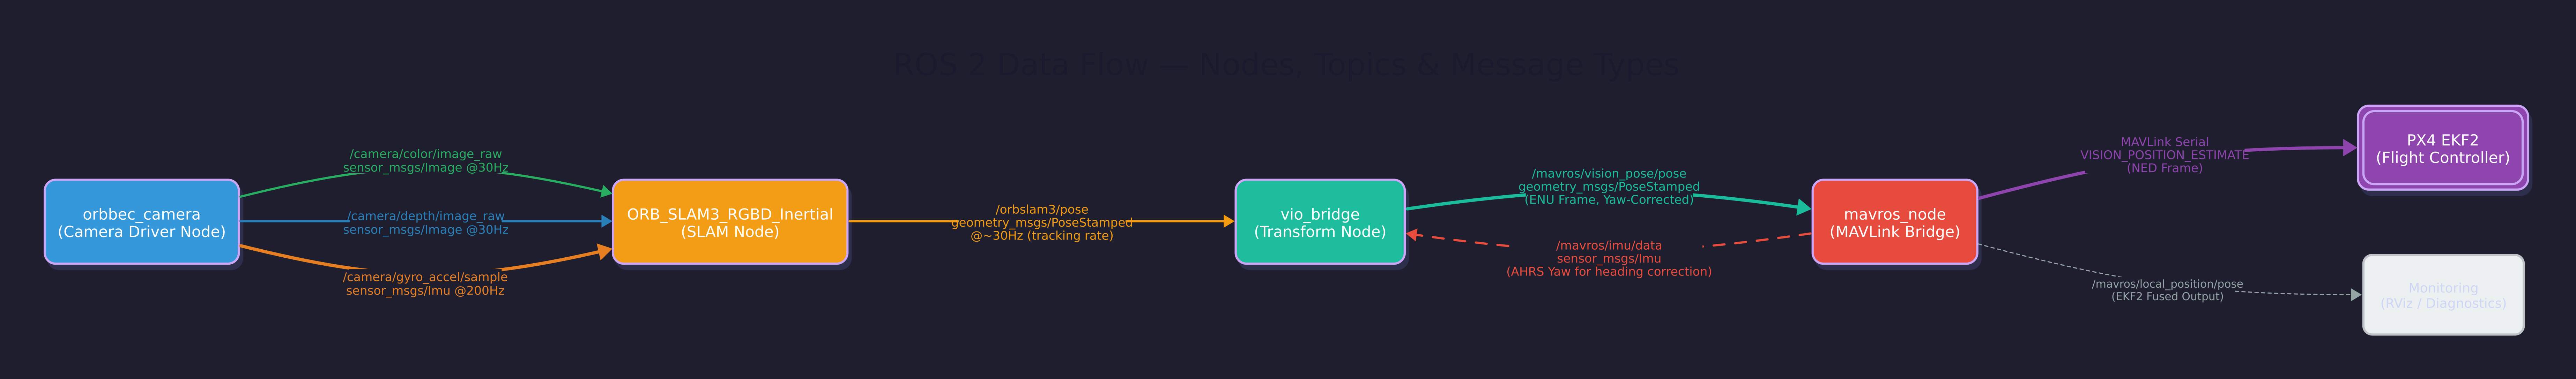
\includegraphics[width=\linewidth,height=0.75\textheight,keepaspectratio]{images/02_ros2_dataflow.jpg}
    \caption{ROS2 Data Flow.}
    \label{fig:data_flow}
\end{figure}

\begin{table}[H]
\centering
\scriptsize % reduces font size
\caption{ROS 2 Sensor Topics}
\resizebox{\textwidth}{!}{%
\begin{tabular}{|p{4.2cm}|p{3.2cm}|p{1.4cm}|p{2.0cm}|p{7.0cm}|}
\hline \textbf{ROS 2 Topic} & \textbf{Message Type} & \textbf{Rate} & \textbf{Resolution} & \textbf{Purpose} \\

\hline /camera/color/image\_raw & sensor\_msgs/Image & 30 Hz & 1280$\times$800 & RGB frames for ORB feature extraction and visual tracking \\

\hline /camera/depth/image\_raw & sensor\_msgs/Image & 30 Hz & 1280$\times$800 & Aligned depth maps for 3D scale estimation (resolves monocular ambiguity) \\

\hline /camera/gyro\_accel/sample & sensor\_msgs/Imu & 200 Hz & N/A & Fused accelerometer + gyroscope for IMU preintegration in ORB-SLAM3 \\

\hline \end{tabular}}
\label{tab:ros2_sensor_topics}
\end{table}

The synchronized accel/gyro output is critical — the camera driver merges both IMU streams into a single topic at 200 Hz, which ORB-SLAM3 buffers and preintegrates between image frames.